\documentclass[english]{his-thesis}

%% Import functionality for front matter, i.e. titlepage and other sections
\usepackage{mattersections}

%%%%%%%%%%%%%%%%%%%%%%%%%%%%%%%%%%%%%%%%%%%%%%%%%%%%%%%%%%%%%%%%%%%%
%% Source code with 'minted'
%%
%% To show source code listings, make use of the 'minted' package.
%% The following lines set some reasonable configuration options.
%% If you do not make use of source code listings in your
%% dissertation, it is safe to remove those lines.

% \usepackage{minted}
% \usepackage{MnSymbol}
% \undef\mathdollar% Remove \mathdollar as defined by MnSymbol to avoid clashes of commands
% \setminted{%
% breaklines,% automatically break longer lines at spaces
% breaksymbolright={\raisebox{-0.4ex}{\ensuremath{\rhookswarrow}}},% show a nice symbol when breaking
% breaksymbolleft={},% no symbol in the continuing line
% breakindent=1em,% indent broken lines' continuation
% linenos=true,% have line numbers
% tabsize=4,% define the width of tab characters
% fontfamily=tt,% use mono-spaced font
% }

%% End of configuration for package 'minted'
%%%%%%%%%%%%%%%%%%%%%%%%%%%%%%%%%%%%%%%%%%%%%%%%%%%%%%%%%%%%%%%%%%%%

%%%%%%%%%%%%%%%%%%%%%%%%%%%%%%%%%%%%%%%%%%%%%%%%%%%%%%%%%%%%%%%%%%%%
%% Custom packages and commands
\usepackage{subcaption, tabularx, xltabular, ccicons, csquotes}
%\usetikzlibrary{arrows,arrows.meta,shapes.arrows,positioning,fit,shapes.geometric,decorations.pathreplacing,calc}

\usepackage[capitalize,noabbrev,nameinlink]{cleveref} % Make use of \cref commands
\creflabelformat{equation}{#1#3#2}
\graphicspath{{img/}{tex/}} % Defines the path to look for images and plots

\usepackage[shortlabels]{enumitem} % Indentation of lists
% Fix indentation for lists.
\setlist[enumerate,1]{leftmargin=0.75cm}
\renewcommand{\arraystretch}{1.5} % Increased vertical space in tables
%% End Custom packages
%%%%%%%%%%%%%%%%%%%%%%%%%%%%%%%%%%%%%%%%%%%%%%%%%%%%%%%%%%%%%%%%%%%%

%%%%%%%%%%%%%%%%%%%%%%%%%%%%%%%%%%%%%%%%%%%%%%%%%%%%%%%%%%%%%%%%%%%%
%% Abbreviations and references
% Abbreviations, will automatically be added to the list of abbreviations if used in the text
% \newacronym{key}{abbreviation}{full name}
\usepackage[acronym,toc=true,nomain,xindy,style=super,nonumberlist,automake]{glossaries-extra}
\setabbreviationstyle[acronym]{long-short}
\makeglossaries
\newacronym{moo}{MOO}{Multi-Objective Optimization}
\newacronym{sbo}{SBO}{Simulation-Based Optimization}
\newacronym{ai}{AI}{Artificial Intelligence}
\newacronym{doe}{DOE}{Design of Experiments}

% Bibliography to use, easiest to include all references, both your own and other sources
%\addbibresource{references.bib}
\addbibresource{example-bibliography.bib}

%% End Abbreviations and references
%%%%%%%%%%%%%%%%%%%%%%%%%%%%%%%%%%%%%%%%%%%%%%%%%%%%%%%%%%%%%%%%%%%%

\usepackage{lipsum} % Only for this example. Remove when starting to write your own.

\begin{document}
% The front matter contains the title page, abstract, abstract in Swedish (Sammanfattning), acknowledgments, your own publications, table of contents, list of figures, list of tables, and abbreviations. 
% The inputs needed are the \thesisabstract, \thesissammanfattning, \thesisacknowledgements, and lastly the ownpublications environment.
\begin{frontmatter}
    \thesisabstract{ % Not more than 360 words (<1 page)
    As society is rapidly changed by electrification, digitalization, and globalization, the automotive industry is particularly affected. Reacting to these changes requires predictive tools, the most common being Discrete-Event Simulation combined with Multi-Objective Optimization, referred to as Simulation-Based Optimization. Production lines are most often the focus for optimization while the factory level is ignored even though the factory level has a larger impact on the total production. One reason for not optimizing on the factory level is the time needed due to the complexity of the line models making up the factory model. This licentiate thesis aims to validate and evaluate a model simplification technique to enable optimization of factories leading to cost and resource effective manufacturing.}

    % Only if dissertation or thesis!
    \thesissammanfattning{\lipsum[1]}
    
    % Acknowledgements if you want to add those.
    \thesisacknowledgements{\lipsum[1]}
    
    % Can be formatted in different ways, see the manual.
    \begin{ownpublications}
    %\highrelevancepublications{fischer2017doctoraldissertationmanual,fischer2017doctoraldissertationmanual}
        %\lowrelevancepublications{}
        %\authorspublication[Authors contribution]{fischer2017doctoraldissertationmanual}
        \authorspublication{fischer2017doctoraldissertationmanual}
        \authorspublication[Design, manuscript preparation, review]{fischer2017doctoraldissertationmanual}
    \end{ownpublications}
\end{frontmatter}

% After the front matter, the main matter of the text is placed, consisting of the contents of the work.
% Recommended to use separate tex files for each chapter organized in subfolders, comment them as necessary to focus on a specific chapter. 
% If not, just include parts, chapters, sections, and subsections as usual.
\part*{Introduction} % Only use parts with doctoral dissertation and licentiate thesis
\chapter{Introduction} \label{chap:introduction}

Some \textbf{interesting} \textsf{introduction} and some \emph{interesting} reference.
\par\textbf{Bold} \textit{Italic} \textbf{\textit{BoldItalic}}
\par\textsf{Sans \textbf{Bold} \textit{Italic} \textbf{\textit{BoldItalic}}}
\par\texttt{Mono \textbf{Bold} \textit{Italic} \textbf{\textit{BoldItalic}}}

\begin{equation}
    \begin{pmatrix}
      1 & 2 & 3  \\
      1 & 2 & 3  \\
      1 & 2 & 3
    \end{pmatrix}
    = \left( \sum_{i=1}^{n-1} i \right)
    = \left( n \right)
\label{eq:first}
\end{equation}

\textcite{Walley2000} writes that \LaTeX\ is really good. \textcite{entrywithurl} agrees. Here's an abbreviation on \gls{ai}. If you want to add additional abbreviations, you can do that in the main file. Here's another abbreviation for \gls{moo}.

To reference figures, tables or sections, use \verb|\cref{label}|, see \cref{tab:citations}, \cref{fig:first_figure}, or the above equation \cref{eq:first}.

\begin{table}
\caption{Various literature citations.}
\begin{tabular}{L{.6\linewidth}L{.3\linewidth}}%
\toprule%
\lstinline|\cite{Walley2000}| & \cite{Walley2000} \\[0.5em]%
\lstinline|\cite{Walley2000,knauth2003prevcompmeasuresshiftwrk,yang2010wikipediacontrib}| & \cite{Walley2000,knauth2003prevcompmeasuresshiftwrk,yang2010wikipediacontrib} \\
\midrule%
\lstinline|\parencite{Walley2000}| & \parencite{Walley2000} \\[0.5em]%
\lstinline|\parencite{Walley2000,knauth2003prevcompmeasuresshiftwrk,yang2010wikipediacontrib}| & \parencite{Walley2000,knauth2003prevcompmeasuresshiftwrk,yang2010wikipediacontrib} \\
\midrule%
\lstinline|\autocite{Walley2000}| & \autocite{Walley2000} \\[0.5em]%
\lstinline|\autocite{Walley2000,knauth2003prevcompmeasuresshiftwrk,yang2010wikipediacontrib}| & \autocite{Walley2000,knauth2003prevcompmeasuresshiftwrk,yang2010wikipediacontrib} \\
\midrule%
\lstinline|\textcite{Walley2000}| & \textcite{Walley2000} \\[0.5em]%
\lstinline|\textcite{Walley2000,knauth2003prevcompmeasuresshiftwrk,yang2010wikipediacontrib}| & \textcite{Walley2000,knauth2003prevcompmeasuresshiftwrk,yang2010wikipediacontrib} \\
\bottomrule%
\end{tabular}%
\label{tab:citations}
\end{table}

\begin{figure}
\centering
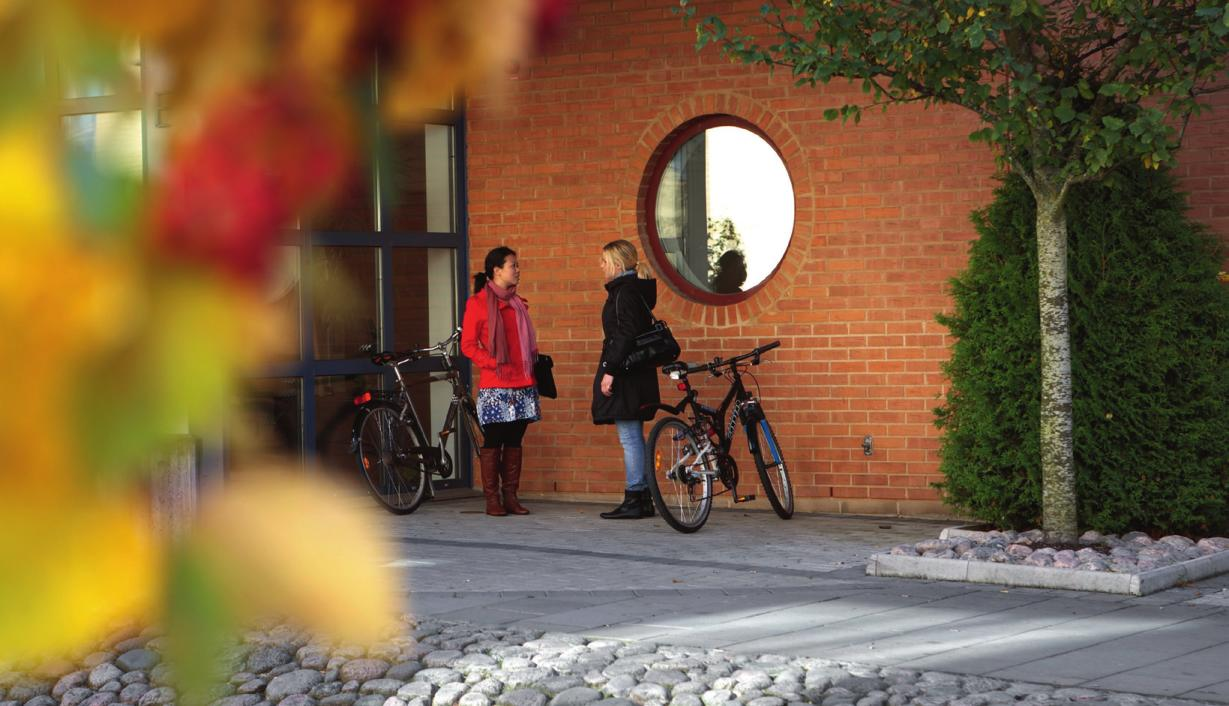
\includegraphics[width=\textwidth]{template/foto.jpg}
\caption{A figure with a long caption. Sed commodo posuere pede. Mauris ut est. Ut quis purus. Sed ac odio.
Sed vehicula hendrerit sem. Duis non odio. Morbi ut dui. Sed accumsan risus eget odio.
In hac habitasse platea dictumst. Pellentesque non elit. Fusce sed justo eu urna porta tincidunt.
Mauris felis odio, sollicitudin sed, volutpat a, ornare ac, erat.}
\label{fig:first_figure}
\end{figure}

Here are examples of a bullet list using the itemize environment:

\begin{itemize}
    \item First item with itemize
    \item Second item
    \item Third item
\end{itemize}

And heres an enumerate environment:

\begin{enumerate}
    \item First item with enumerate
    \item Second item
    \item Third item
\end{enumerate}

If you need footnotes, use the \verb|\footnote{}| command and they will appear looking like this\footnote{This is a footnote.}.

\lipsum[6-8]

\section{Outline}
\label{sec:outline}

\lipsum[11]

\part*{Frame of Reference}
% Literature review
\chapter{Frame of Reference} \label{chap:frameofreference}
\lipsum[13-14]

\section{The Method}

\lipsum[1]

\begin{equation}
\label{eq_the_method}
    f(x) = x_1^2 + x + 1
\end{equation}

\lipsum[2]

\subsection{More Details}

More references here \cite{krishnamurthy2003manageroverview,dedrick2006scope,henkel2006revealingemblinux,fitzgerald2003trencheslessons, entrywithurl}.

\lipsum[15-19]

\part*{Research Methodology}
% Philosophical paradigm and research strategy
\chapter{Research Methodology} \label{chap:methods}
\lipsum[12-18]

\part*{Summary of Included Papers}
% Results, main contributions and summary for each source
\chapter{Summary of Included Publications} \label{chap:results}
\lipsum[3]

\section{Paper I}
\lipsum[1]

\section{Paper II}
\lipsum[2]

\part*{Conclusions}
% Summary and final remarks (Conclusions)
\chapter{Conclusions and Future Work} \label{chap:summary}
As seen in \cref{chap:results} this dissertation is full of interesting results.
\lipsum[20-25]

\section{Conclusions}
\lipsum[20-25]

\section{Further work}
\lipsum[20-25]

% Start of back matter, appendix, list of references, included full text articles, and list of previous dissertations
% List of references and list of previous dissertations are automatically placed using the backmatter environment, only the fullarticles environment is needed.
\begin{backmatter}
    % Example of including full text articles in the manuscript.
    % It's possible to specify what is written both before the reference and after.
    % \fullarticle[includepdf options]{reference}{pdf-file}[before][after]
    \begin{fullarticles}
        \fullarticle[scale=.9,trim={0mm 5mm 0mm 5mm},pages=-]{fischer2017doctoraldissertationmanual}{manual.pdf}[\href{https://creativecommons.org/licenses/by-nc-nd/4.0/}{\ccbyncnd}]
        \fullarticle[scale=.9,trim={0mm 5mm 0mm 5mm},pages=1]{fischer2017doctoraldissertationmanual}{manual.pdf}[\copyright{} 2018 University of Skövde. Reprinted, with permission, from]
        \fullarticle[scale=.9,trim={0mm 5mm 0mm 5mm},pages=1]{fischer2017doctoraldissertationmanual}{manual.pdf}[Reprinted from][with permission from University of Skövde.]
    \end{fullarticles}
\end{backmatter}
\end{document}
